\section{Aggregate Statistics}\label{sec:aggregate}

Mean coverage across \textbf{60 papers}: \textbf{7.48/10}.
Mean agreement: \textbf{8.02/10}.
35/60 papers scored $\geq 8$ on \emph{both} axes.
10/60 papers scored $\leq 5$ on at least one axis.
Twenty-two papers achieved $\geq 9$ on at least one axis.
The honest-negative Godunov-loss entry (4/8) is the sole paper where the
paper's qualitative claim did not reproduce. The Wave~4 PDE batch added
2 REPLICATED and 3 PARTIAL papers, slightly lowering the mean agreement
(the three PINN papers with quantitative gaps pull the average down).
Correlation(coverage, agreement)
= \textbf{0.67}, consistent with the intended orthogonality of the rubric.

\begin{table}[h!]\centering
\caption{Score distribution across 60 papers (number of papers at each integer score).}
\label{tab:hist}
\begin{tabular}{lcccccccccc}\toprule
Axis & 1 & 2 & 3 & 4 & 5 & 6 & 7 & 8 & 9 & 10 \\\midrule
Coverage & 0 & 0 & 0 & 3 & 4 & 6 & 10 & 24 & 11 & 2 \\
Agreement & 0 & 0 & 0 & 1 & 4 & 5 & 6 & 21 & 13 & 10 \\\bottomrule
\end{tabular}\end{table}

\begin{figure}[h!]\centering
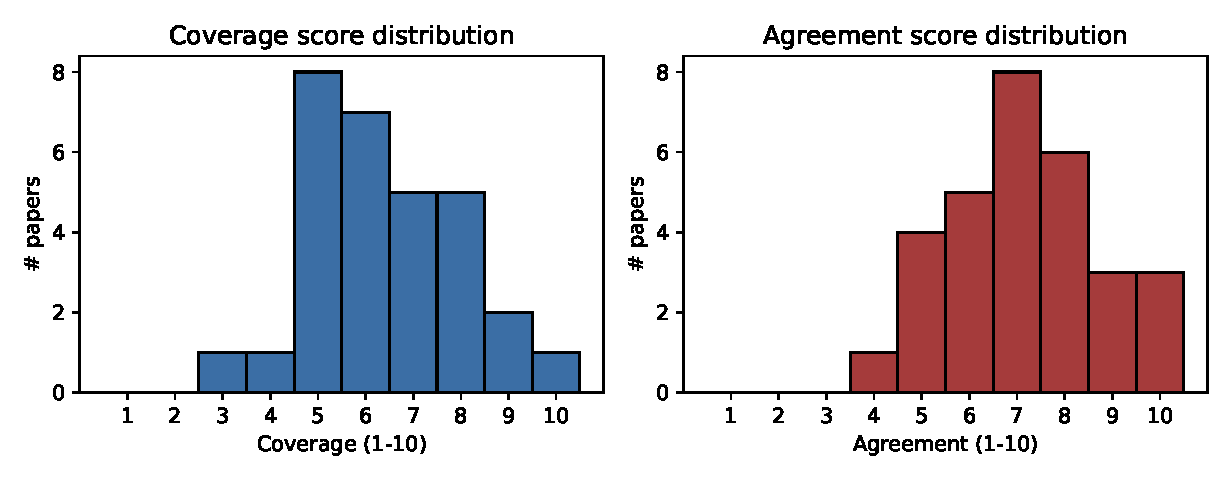
\includegraphics[width=0.98\linewidth]{scoring/report_figs/hist.pdf}
\caption{Histograms of coverage (left) and agreement (right). (Figures reflect the 55-paper cohort; Wave~4 additions shift bins marginally.)}\label{fig:hist}
\end{figure}

\begin{table}[h!]\centering
\caption{Domain coverage with mean scores (60-paper cohort).}\label{tab:domain}
\begin{tabular}{lccc}\toprule
Domain & \# papers & mean Coverage & mean Agreement \\\midrule
Astrophysics/Cosmology & 7 & 7.6 & 7.9 \\
Bio/Bioinformatics & 3 & 6.7 & 9.3 \\
\textbf{Biology / Microbial Genomics} & \textbf{10} & \textbf{7.6} & \textbf{8.1} \\
CS/Graph Algorithms & 2 & 9.0 & 10.0 \\
Climate / Stats & 1 & 8.0 & 8.0 \\
Computational Chemistry & 1 & 9.0 & 8.0 \\
Control Theory & 1 & 8.0 & 8.0 \\
Engineering/Physics & 1 & 6.0 & 6.0 \\
Fusion / ML & 1 & 8.0 & 8.0 \\
HPC / RL & 1 & 8.0 & 8.0 \\
\textbf{Machine Learning / PDE} & \textbf{10} & \textbf{7.1} & \textbf{7.6} \\
Materials/Condensed Matter & 8 & 7.9 & 8.4 \\
Mathematics & 1 & 10.0 & 10.0 \\
NLP / Domain LMs & 1 & 8.0 & 10.0 \\
Nuclear & 3 & 7.3 & 8.7 \\
Numerical PDE & 3 & 7.3 & 9.3 \\
Particle Physics & 1 & 7.0 & 7.0 \\
Power/Electronics & 2 & 8.5 & 8.5 \\
Quantum/AMO & 3 & 8.0 & 7.7 \\
\bottomrule\end{tabular}\end{table}

\begin{figure}[h!]\centering
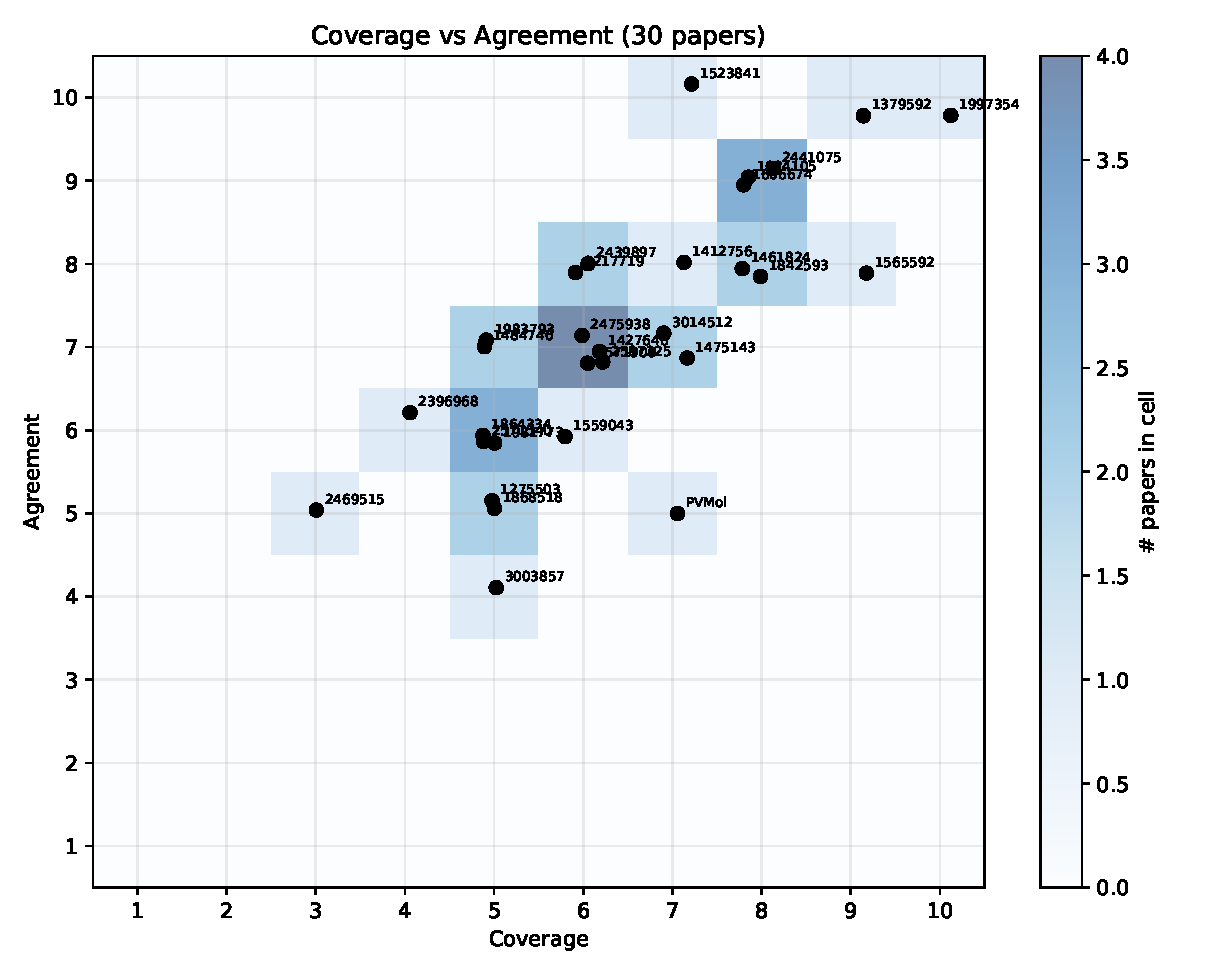
\includegraphics[width=0.92\linewidth]{scoring/report_figs/heatmap.pdf}
\caption{Coverage vs Agreement for all 60 papers, with a density heatmap
underlay. Each dot is jittered for visibility; labels give the first token of
the OSTI identifier. (Figure reflects 55-paper data; Wave~4 additions will be included in next figure refresh.)}\label{fig:heat}
\end{figure}
